\subsection{Design Goals}
\label{rasc:sec:properties}

We discuss \Cref{rasc:tab:properties}'s key goals in detail.

\noindent \textbf{Action progress updates.} 
This goal implies that
the primitive should provide feedback at key points of the action execution: acknowledgment, action start, and action end (and if the device supports it, during the action). Doing so may require polling, and this polling needs to be efficient. 


\noindent \textbf{Action failure detection.} When an action fails, the primitive should detect it quickly.
This property may be implemented atop RPC-complete with the use of a timeout after the expected action length is over; however, that is not trivial since there is no fixed length for each action.

\begin{figure}[tb]
    \begin{subfigure}[t]{0.48\linewidth}
        \centering
        {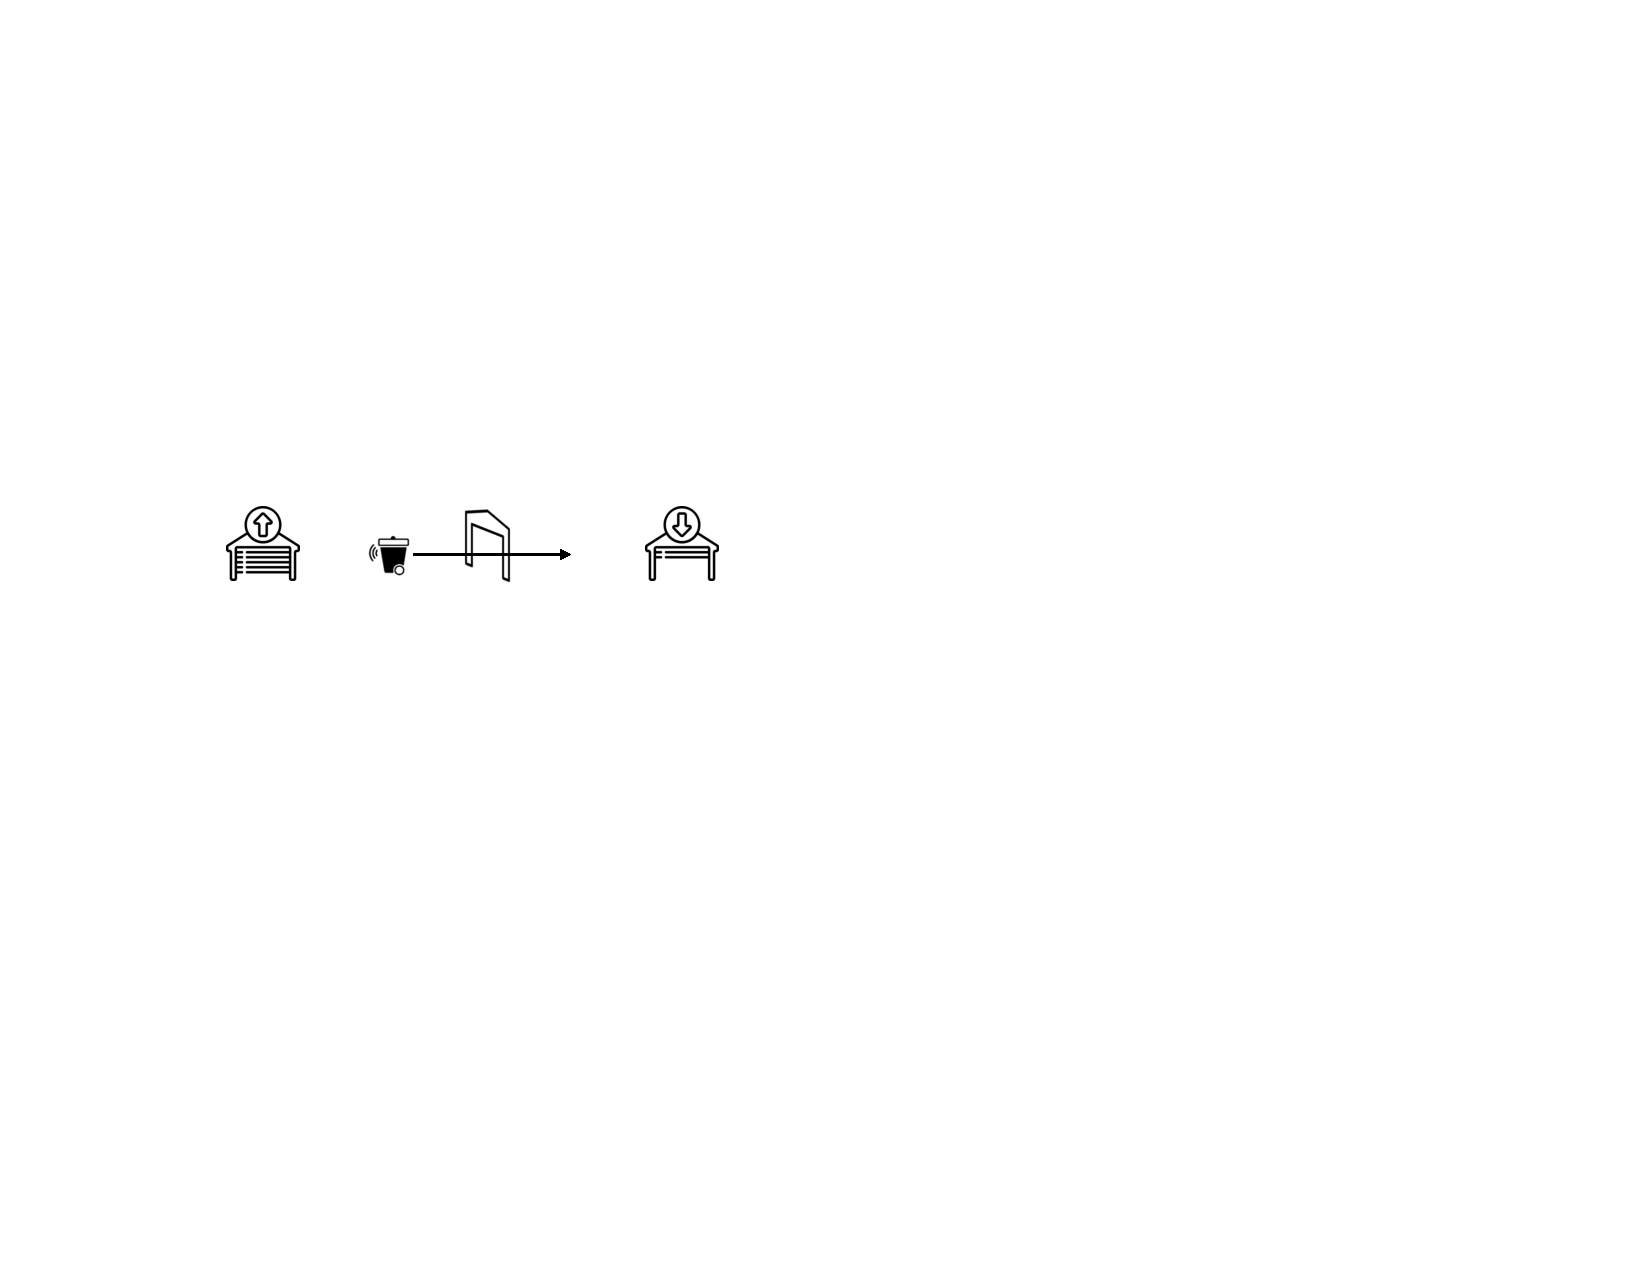
\includegraphics[width=0.95\textwidth]{RASC/figures/intro/garage-routine-desc.pdf}}
        \caption{\small \textit{Routine description:} (i) the garage door opens; (ii) the trashcan is moved out into the driveway; (iii) the garage door closes.}
        \label{rasc:fig:garage-routine-desc}
    \end{subfigure}
    \hfill
    \begin{subfigure}[t]{0.47\linewidth}
        \centering
        {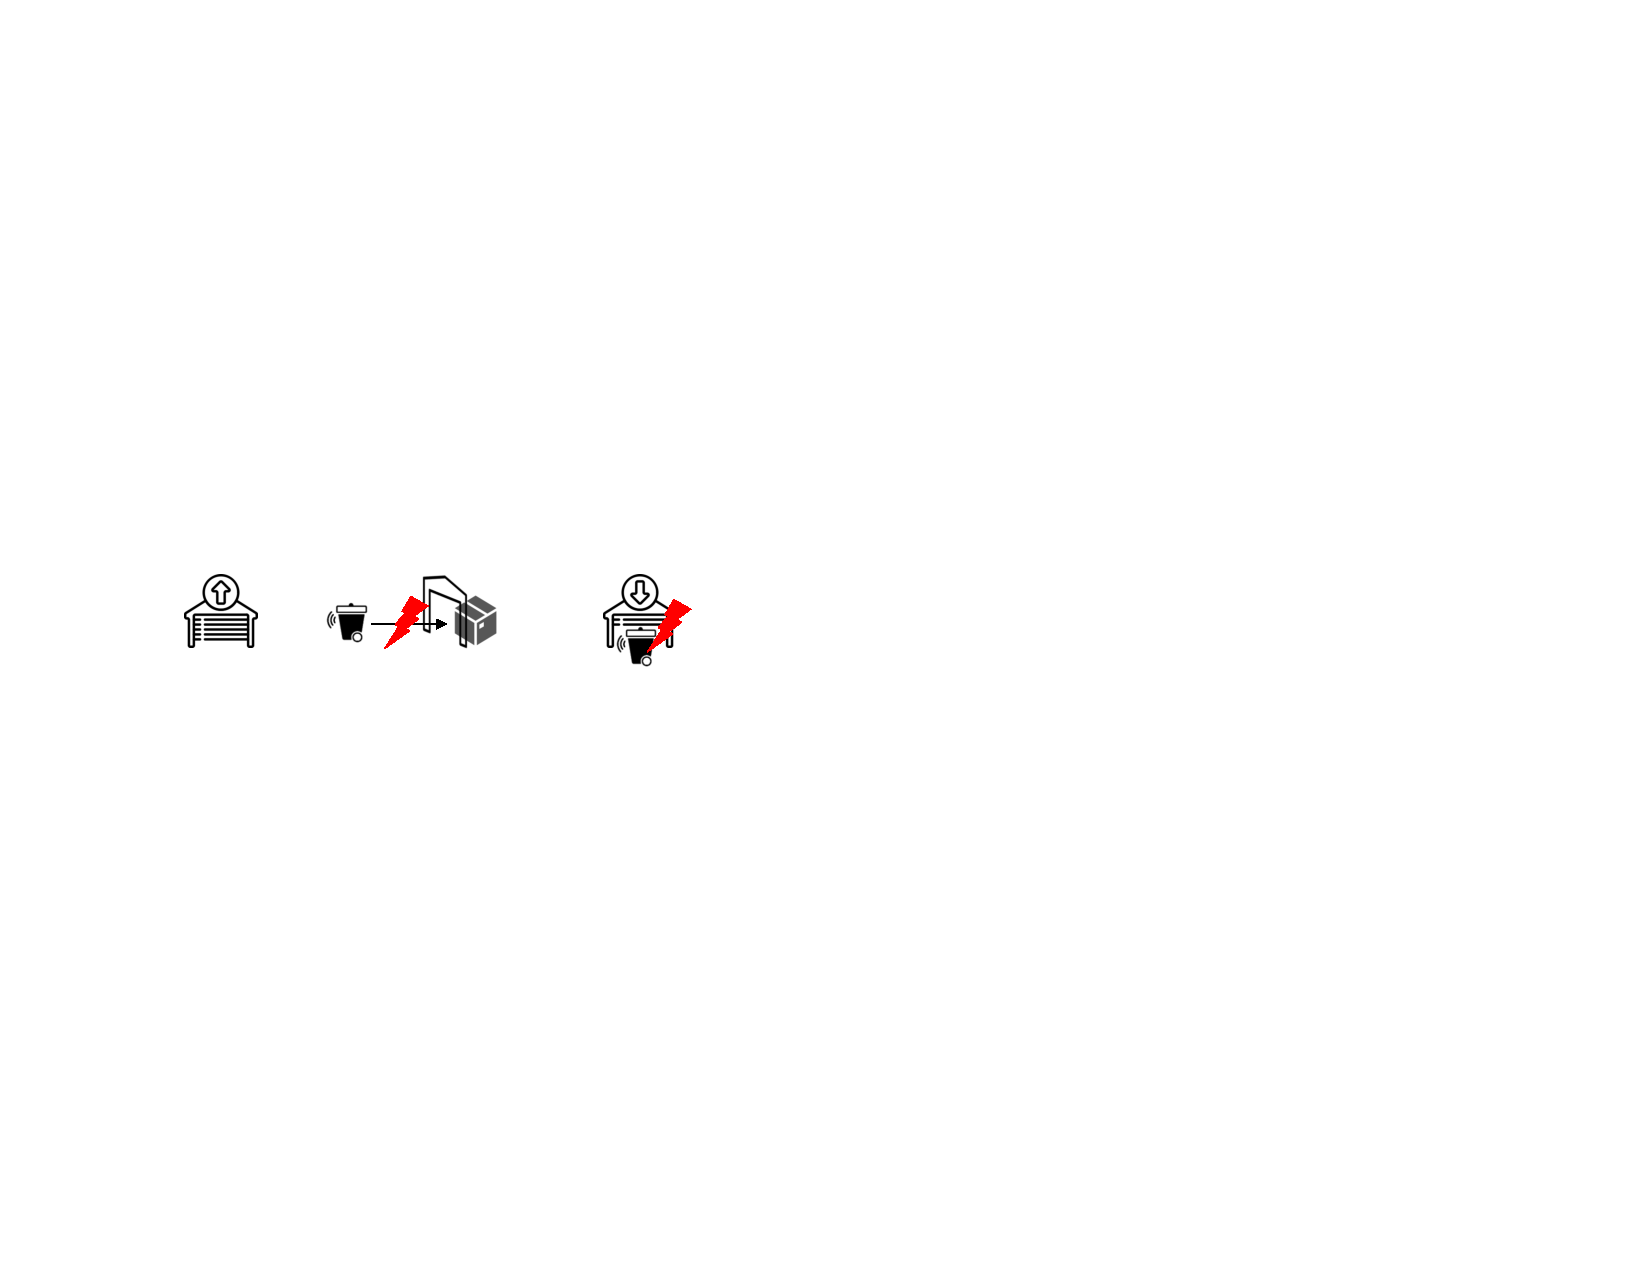
\includegraphics[width=\linewidth]{RASC/figures/intro/garage-routine-failure.pdf}}
        \caption{\small \textit{Action failures:} the trashcan gets stuck below the garage door because of an obstacle and the garage door cannot close.}
        \label{rasc:fig:garage-routine-failure}
    \end{subfigure}
    \par\medskip
    \begin{subfigure}[t]{0.48\linewidth}
        \centering
        {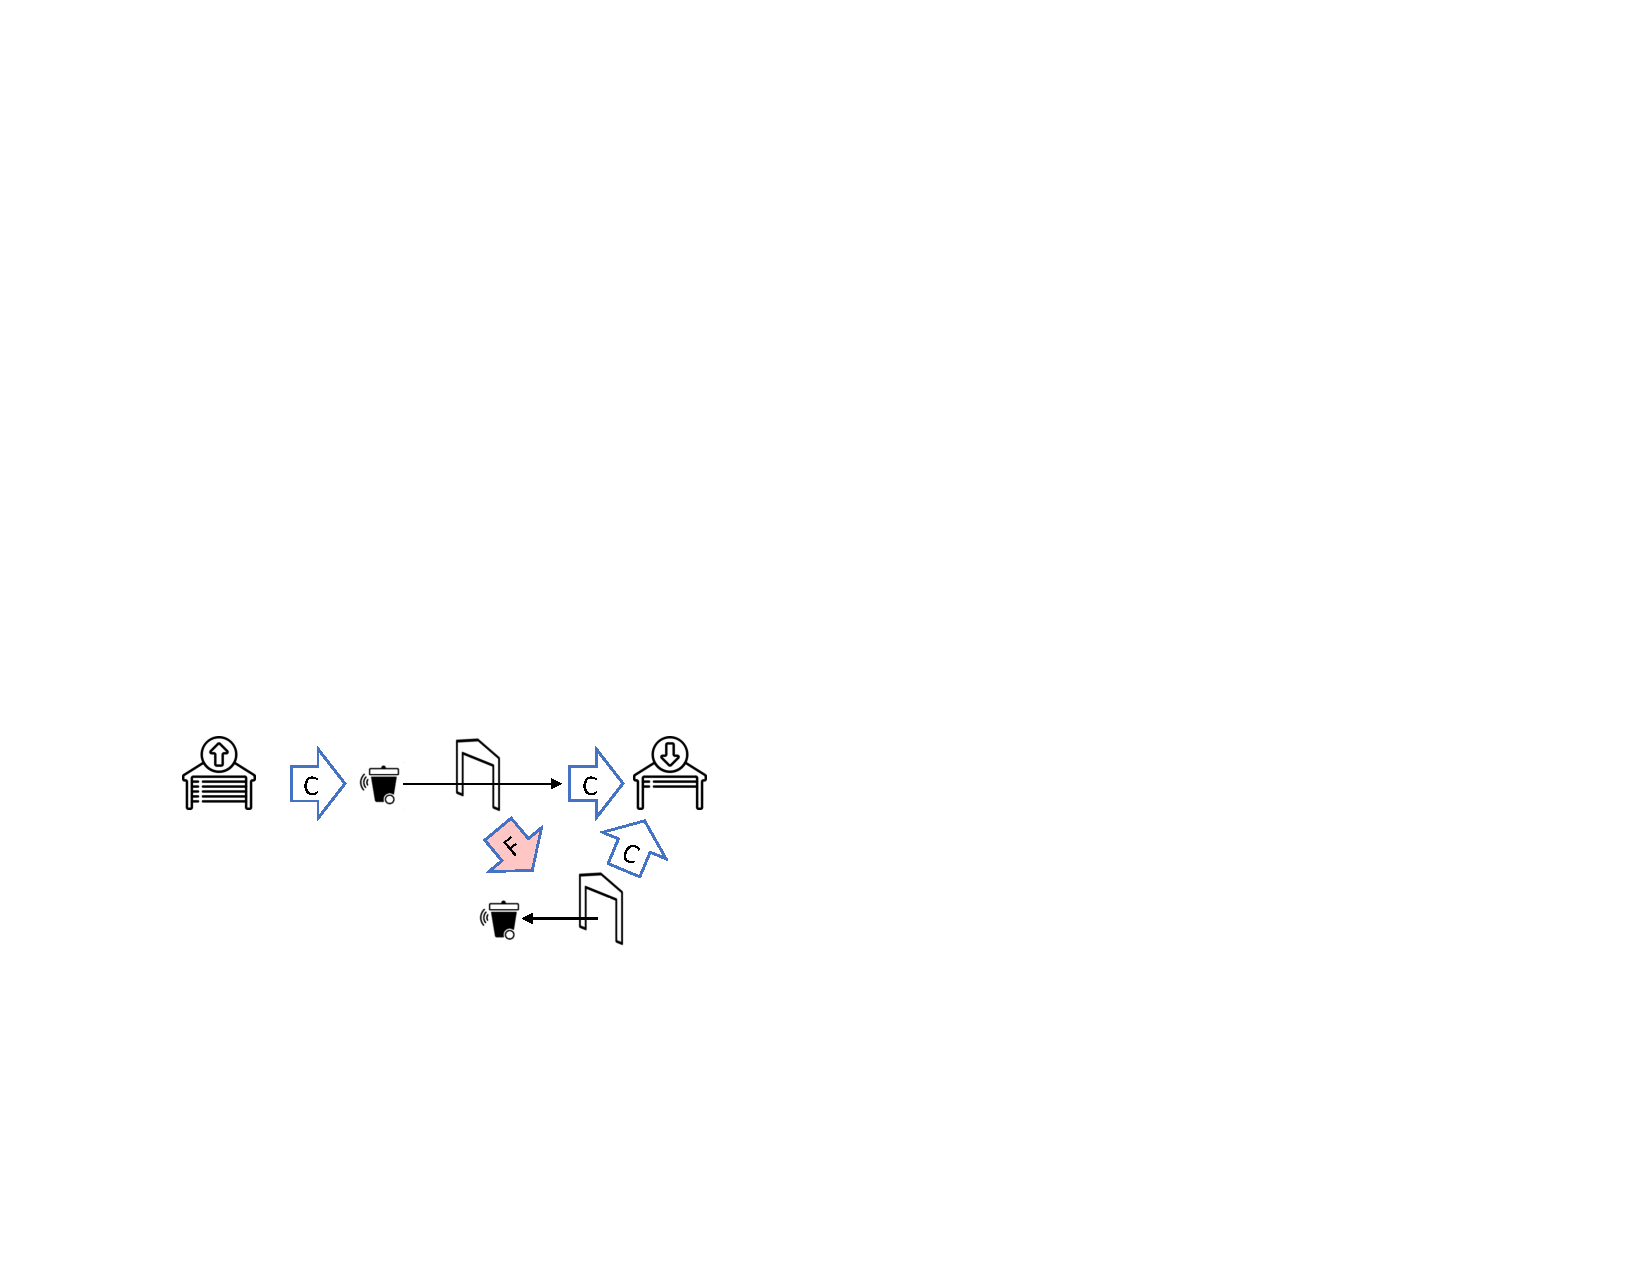
\includegraphics[width=\textwidth]{RASC/figures/intro/garage-routine-fallback.pdf}}
        \caption{\small \textit{Fallback actions:} the trashcan moves back inside after the first movement's failure and the garage door closes.}
        \label{rasc:fig:garage-routine-fallback}
    \end{subfigure}
    \hfill
    \begin{subfigure}[t]{0.47\linewidth}
        \centering
        {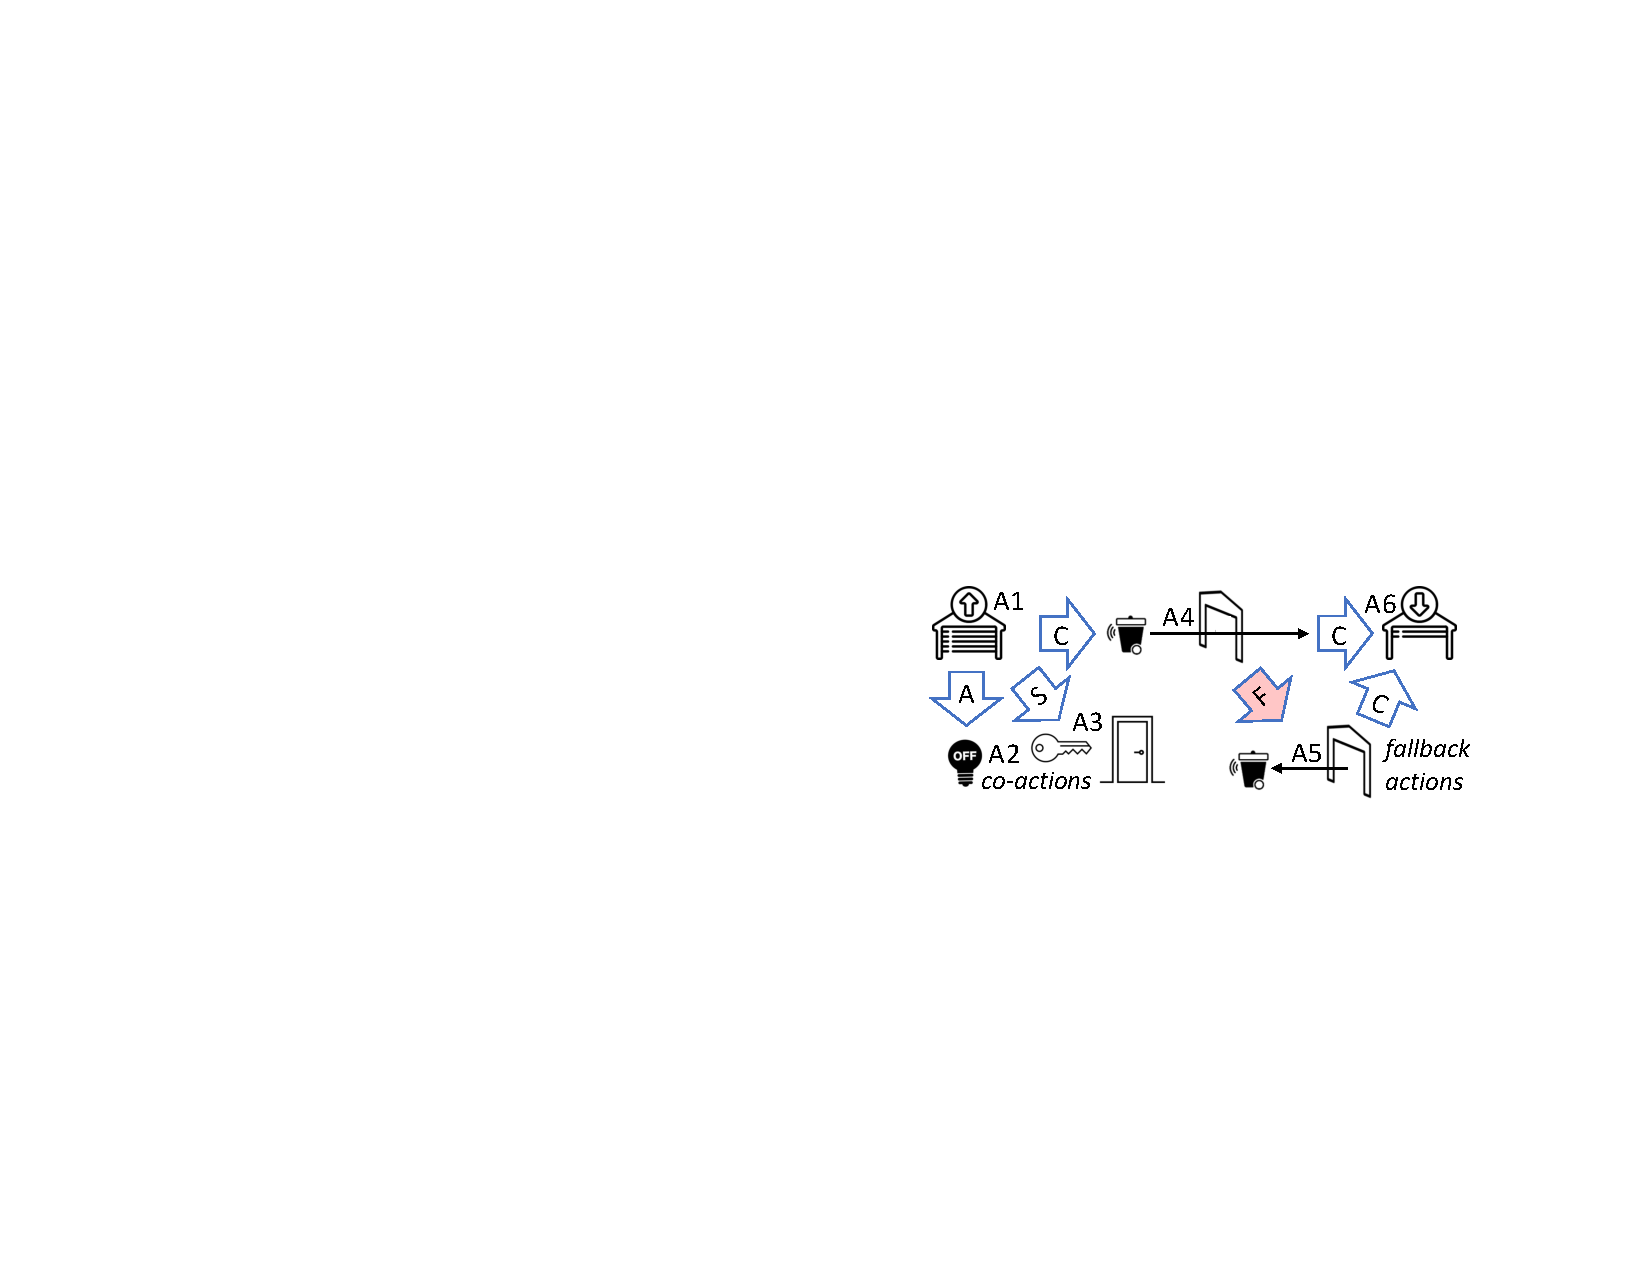
\includegraphics[width=\textwidth]{RASC/figures/intro/garage-routine-workflow.pdf}}
        \caption{\small \textit{Routine as a workflow:} diverse action dependencies allow for fine-grained control with \textit{co-actions} and \textit{fallback actions}.
        }
        \label{rasc:fig:garage-routine-workflow}
    \end{subfigure}
    \caption{\small \textbf{Routine with exception handling. {\it Garage door opens, automatic trash can~\cite{smartcan_protolabs}
    goes out, garage door closes. Letter inside arrow indicates trigger event: S=Start, C=Complete, F=Failure.}
    }}
    \label{rasc:fig:garage-routine}
\end{figure}

\noindent \textbf{Diverse action dependencies.}
The primitive must support rich inter-action dependencies. For a given example (garage door opens and closes for a trashcan
), \Cref{rasc:fig:garage-routine}(a,b) show two scenarios, and \Cref{rasc:fig:garage-routine}(c,d) show two variants. 
In \Cref{rasc:fig:garage-routine-workflow},
$A2$ and $A3$ are \textit{co-actions} of
$A1$. The co-action concept allows (i) the light to turn off {\it before} the garage door starts opening, so that insects are not drawn indoors, and (ii) the inside door to lock only if the garage door starts opening; 
if $A1$ fails, no safety gap occurs.
If $A4$ \textit{fails}
(\Cref{rasc:fig:garage-routine-failure}), the \textit{fallback action} $A5$ returns the trashcan
to its original spot, and, finally, $A6$ closes the garage door
to prevent exposure to robbers. 
Implementing \Cref{rasc:fig:garage-routine-workflow} via RPC 
requires users stitching multiple routines 
(roughly four here--one extra for every new dependency type) guarded by complex predicates to emulate progress points, 
to block unintended triggers. This is prohibitive.  

\noindent \textbf{Dynamic action scheduling.}
When action lengths differ from the schedule, the primitive should reschedule subsequent actions. 
Previous smart home routine scheduling~\cite{SafeHomeEuroSys2021} 
(\Cref{rasc:fig:garage-routine-desc}) ignores 
unbounded action lengths and diverse dependencies (\Cref{rasc:fig:energy-saving-vacuum-rasc,rasc:fig:garage-routine-workflow}), relying instead on static schedules. 
Action durations are context-dependent (e.g., 
floor area, dirt level for vacuum, etc.), and failures are unpredictable at compile or schedule time. 
The schedule must adapt to ensure: (a) \textit{safety}, i.e.,
no actions trigger concurrently for the same device
(which might cause 
action rejections),  (b) upheld action dependencies, and (c) 
early starts for actions if predecessors finish ahead of schedule.
\RPCa{} and \RPCs{} cannot handle this, and \RPCc{} only detects completion. 
\abstraction{} is more powerful.